% Schematic figures for the report: (1) the capture->train->infer pipeline,
% (2) the kernel-predicting (KPCN) output head.
%
% Compile to two cropped PDFs (one per tikzpicture) with:
%     pdflatex schematics.tex
% Produces schematics.pdf (page 1 = pipeline, page 2 = KPCN head). Use
% \includegraphics[page=1]{schematics} / [page=2] in the report, or split with
% `pdfseparate schematics.pdf fig-%d.pdf`.
%
% If you prefer to draw these in Excalidraw/draw.io instead, the box/arrow
% layout below doubles as a spec.

\documentclass[tikz,border=6pt,multi=tikzpicture]{standalone}
\usepackage{tikz}
\usetikzlibrary{arrows.meta,positioning,fit,backgrounds,calc}

\tikzset{
  box/.style={draw,rounded corners=2pt,minimum height=9mm,minimum width=20mm,
    align=center,font=\small,fill=blue!4},
  data/.style={draw,rounded corners=2pt,minimum height=8mm,align=center,
    font=\footnotesize,fill=gray!8},
  net/.style={draw,rounded corners=3pt,minimum height=12mm,minimum width=24mm,
    align=center,font=\small\bfseries,fill=blue!12},
  ours/.style={draw,rounded corners=3pt,minimum height=12mm,minimum width=24mm,
    align=center,font=\small\bfseries,fill=orange!18},
  flow/.style={-{Stealth[length=2.5mm]},thick},
  tflow/.style={-{Stealth[length=2.5mm]},thick,dashed,gray},
}

\begin{document}

% =========================================================================
% Figure 1: pipeline (capture -> train/infer)
% =========================================================================
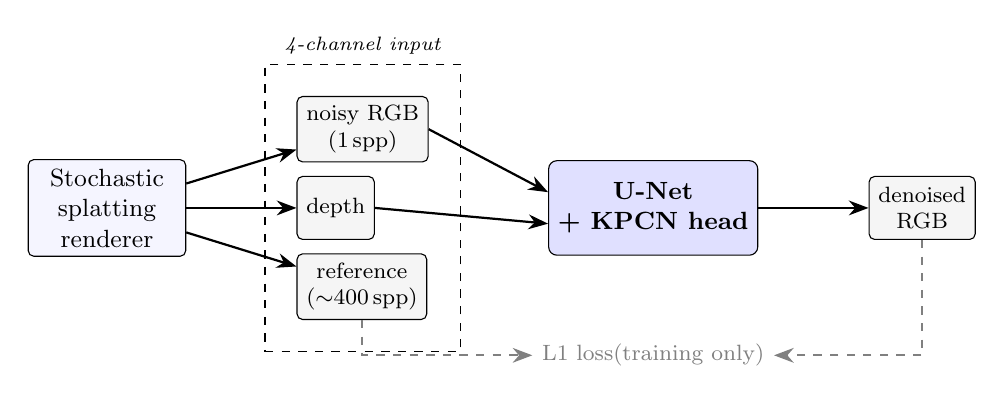
\begin{tikzpicture}[node distance=7mm and 14mm]
  \node[box] (rend) {Stochastic\\splatting\\renderer};

  \node[data,right=of rend,yshift=10mm] (noisy) {noisy RGB\\(1\,spp)};
  \node[data,right=of rend]              (depth) {depth};
  \node[data,right=of rend,yshift=-10mm] (clean) {reference\\($\sim$400\,spp)};

  \node[net,right=22mm of depth] (unet) {U-Net\\+ KPCN head};
  \node[data,right=of unet] (out) {denoised\\RGB};

  \draw[flow] (rend) -- (noisy);
  \draw[flow] (rend) -- (depth);
  \draw[flow] (rend) -- (clean);

  % 4-channel input (noisy RGB + depth) into the network
  \draw[flow] (noisy.east) -- ($(unet.west)+(0,2mm)$);
  \draw[flow] (depth.east) -- ($(unet.west)-(0,2mm)$);
  \draw[flow] (unet) -- (out);

  % training-only supervision arrow from reference to a loss
  \node[font=\footnotesize,gray,below=10mm of unet] (loss) {L1 loss\\(training only)};
  \draw[tflow] (clean.south) |- (loss.west);
  \draw[tflow] (out.south) |- (loss.east);

  \begin{scope}[on background layer]
    \node[draw,dashed,inner sep=4mm,fit=(noisy)(depth)(clean),
      label={[font=\scriptsize\itshape]above:4-channel input}] {};
  \end{scope}
\end{tikzpicture}

% =========================================================================
% Figure 2: kernel-predicting (KPCN) output head
% =========================================================================
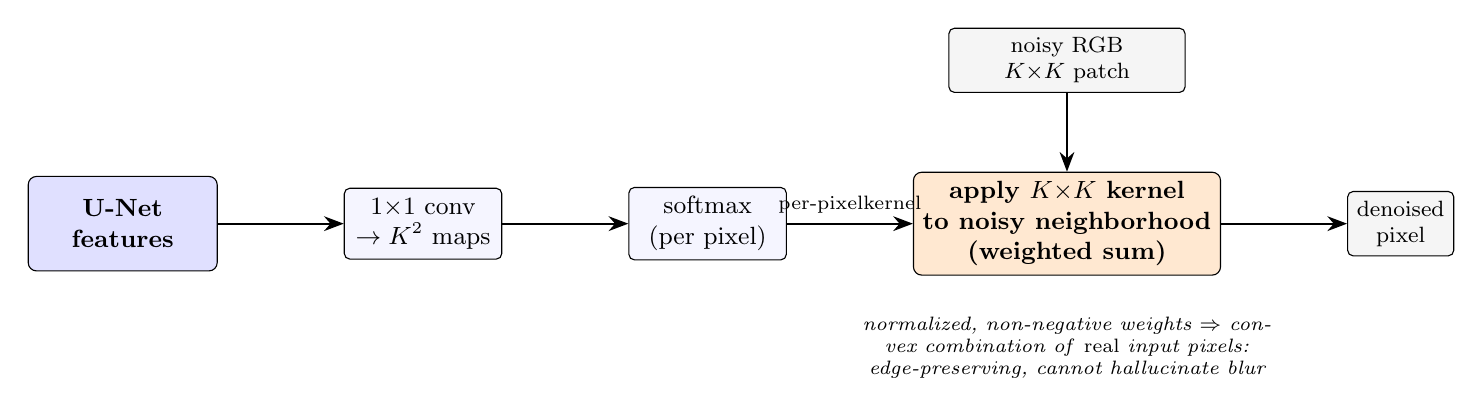
\begin{tikzpicture}[node distance=8mm and 16mm]
  \node[net] (feat) {U-Net\\features};
  \node[box,right=of feat] (conv) {$1{\times}1$ conv\\$\rightarrow K^2$ maps};
  \node[box,right=of conv] (soft) {softmax\\(per pixel)};
  \node[ours,right=of soft,minimum width=30mm] (apply)
    {apply $K{\times}K$ kernel\\to noisy neighborhood\\(weighted sum)};
  \node[data,right=of apply] (out) {denoised\\pixel};

  \node[data,above=10mm of apply,minimum width=30mm] (noisy)
    {noisy RGB\\$K{\times}K$ patch};

  \draw[flow] (feat) -- (conv);
  \draw[flow] (conv) -- (soft);
  \draw[flow] (soft) -- node[font=\scriptsize,above]{per-pixel\\kernel} (apply);
  \draw[flow] (noisy) -- (apply);
  \draw[flow] (apply) -- (out);

  \node[font=\scriptsize\itshape,below=4mm of apply,text width=58mm,align=center]
    {normalized, non-negative weights $\Rightarrow$ convex combination of
     \emph{real} input pixels: edge-preserving, cannot hallucinate blur};
\end{tikzpicture}

\end{document}
